\documentclass[12pt]{article}
%--------------------   start of the 'preamble'
%
\usepackage{graphicx,amssymb,amstext,amsmath,color}
\usepackage{grffile}
\usepackage[margin=2cm]{geometry}
\usepackage{abstract}
\usepackage{setspace}
\usepackage[footnotesize,bf]{caption}

% TABLE
\usepackage{multicol,hhline,colortbl,multirow}
\usepackage{braket}
\usepackage{siunitx}
\usepackage{hyperref}
\usepackage{authblk}
\usepackage{siunitx}
\usepackage{adjustbox}
\usepackage{mathrsfs}
%%\usepackage[sort&compress]{natbib}
%%\bibpunct{(}{)}{,}{a}{, }{;}
%
\usepackage[sort&compress]{natbib}
\bibpunct{[}{]}{,}{s}{}{;}


\definecolor{gray}{gray}{0.8}
\def\mobunits{\square\centi\meter\per\volt\per\second}
\def\gcm{\gram\per\cubic\centi\meter}
\def\ccg{\cellcolor{gray}}

\renewcommand{\labelitemii}{$\circ$}
\renewcommand{\bibname}{References}


\title{MorphCT Results - Disabling Gaussian Mapping}
\author{Matthew Jones}
\date{\today}

\begin{document}
\maketitle


\section{What effects have the recent changes to the neighbourlist and finegraining processes had on our ability to predict the morphology without performing a Gaussian mapping on our predicted chromophore density of states?}


\subsection{In a line}

Currently inconclusive.

\subsection{Explanation}


It's been a while since we considered the Gaussian mapping that is performed on the chromophore HOMO/LUMO levels in order to reduce their standard deviation.
Usually we `squeeze' the distribution down to $\sim$ 100 meV, which is the value predicted from experiment.
This reduce $\Delta E_{ij}$ in the hopping rate equation closer to the $\lambda_{ij}$, which permits faster rates and quicker hops.
However, recently, we have made several changes to the fine-graining and neighbourlist generation procedures, so perhaps the Gaussian mapping (which could be regarded as somewhat arbitrary) is no longer necessary.

To test this hypothesis, we perform simulations of our classic neat P3HT systems equilibrated at 5 temperature state points and examine their mobilities when the DoS have not been modified.

The current data shows that we still need to perform the Gaussian mapping in order to get sensible mobility trends, however there are issues with the qualitative trend, and until these are addressed, we cannot say this with any certainty.

\clearpage

\subsection{No Gaussian Mapping Results}


\begin{figure}[h!]\centering
	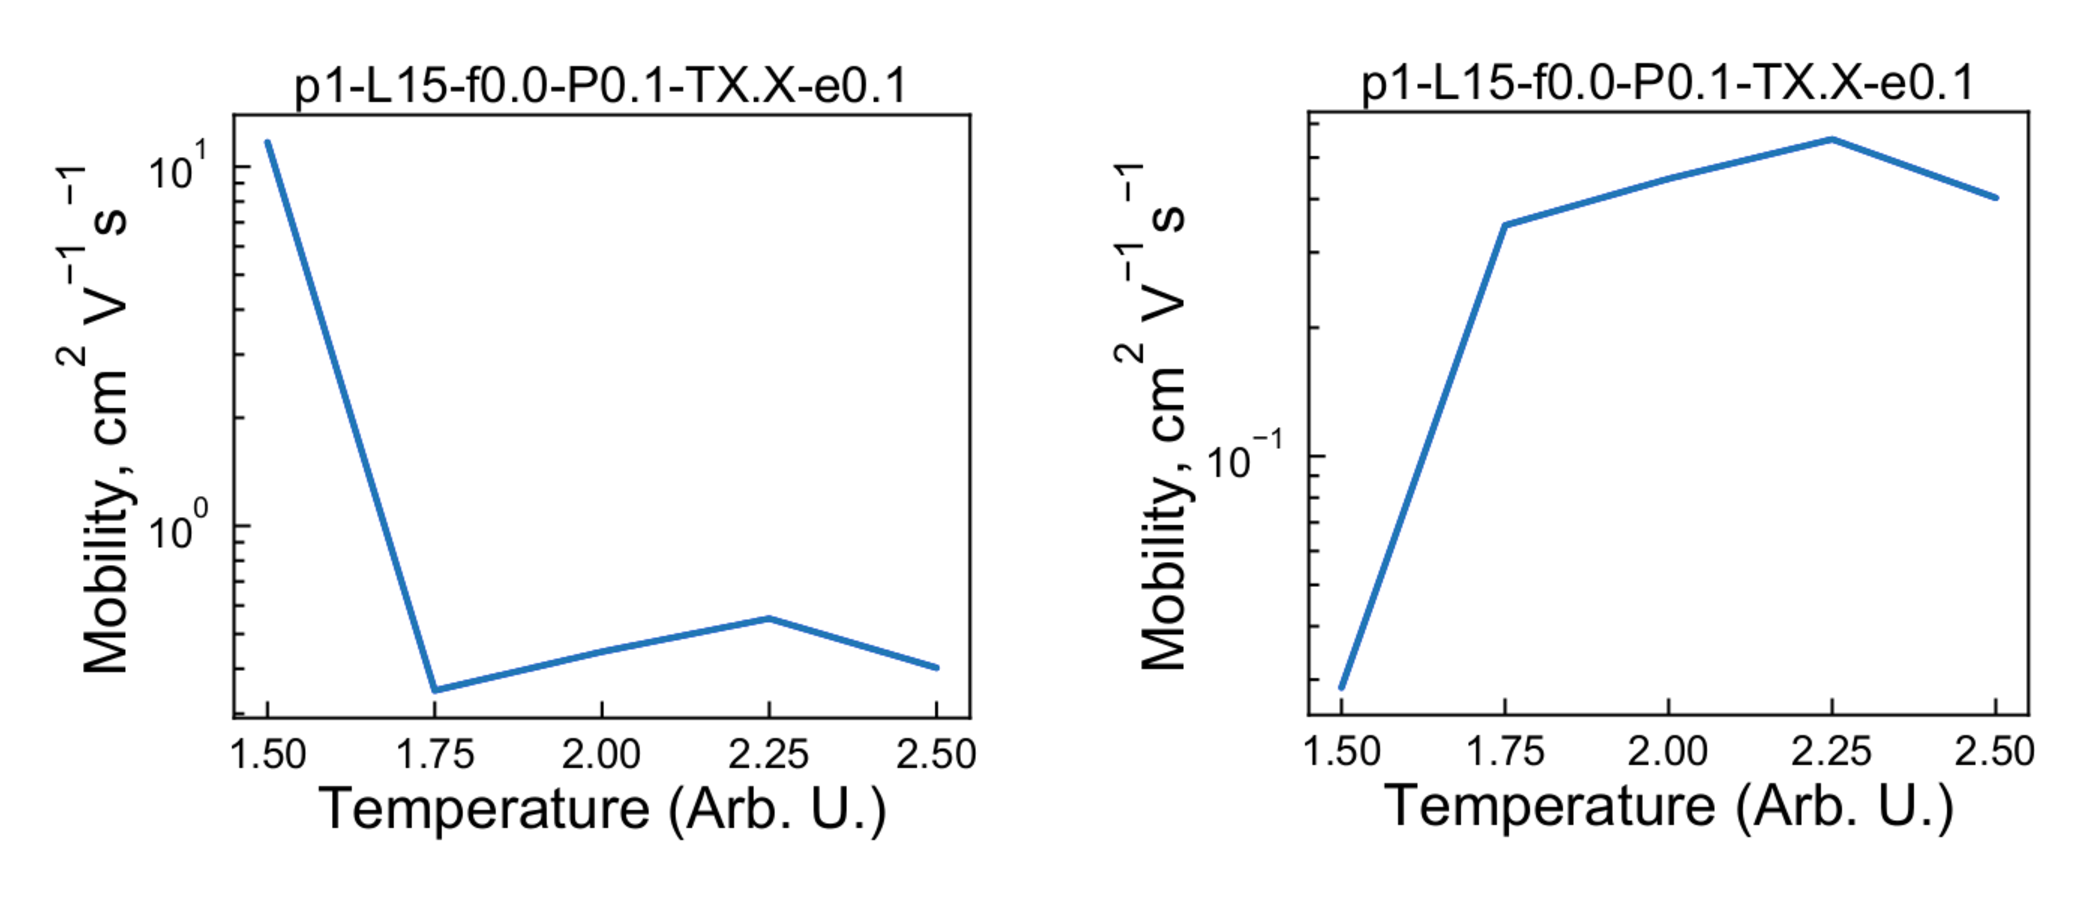
\includegraphics[width=\textwidth]{Figures/mobilityHole.pdf}
    \caption{The evolution of the mobility for the neat P3HT state points with the Gaussian mapping disabled.
        Left: With Gaussian Mapping shrinking the DoS sigma to 100 meV.
        Right: Without Gaussian Mapping, taking the DoS as produced from ORCA.
}
	\label{fig:Mobility}
\end{figure}


Figure \ref{fig:Mobility} shows the differences in the mobility curves when the HOMO distribution has and has not been Gaussian mapped.
The trend is clearly incorrect.
The ordered system is reporting an order of magnitude \textit{LOWER} mobilities than the disordered systems.
One interesting thing to note is that there doesn't appear to be a significant difference in the reported mobilities for the disordered morphologies.
\textcolor{red}{In fact, the mobilities are identical. 
    This surprises me greatly, and makes me think that MorphCT was again storing previous data. 
    I really need to work out if/why this is, as the log files show a complete pipeline run with no previously saved data.
    I'm rerunning this on Fry from the top to see if the results change.
}

\textcolor{blue}{Additionally, it looks like the T1.5 and T1.75 simulations did not obtain sufficient data to get good fits to the MSD of the system.
This manifests in figures \ref{fig:noMapT1.5} and \ref{fig:noMapT1.75} as poor MSD fits in \textbf{10)}, \textbf{11)}, and \textbf{12)}, as well as insufficient carrier transport shown in the anisotropy figures \textbf{5)}.
To remedy this, I am running a larger number of carriers over longer KMC simulation time to see if this helps.
}


\begin{figure}[h]\centering
	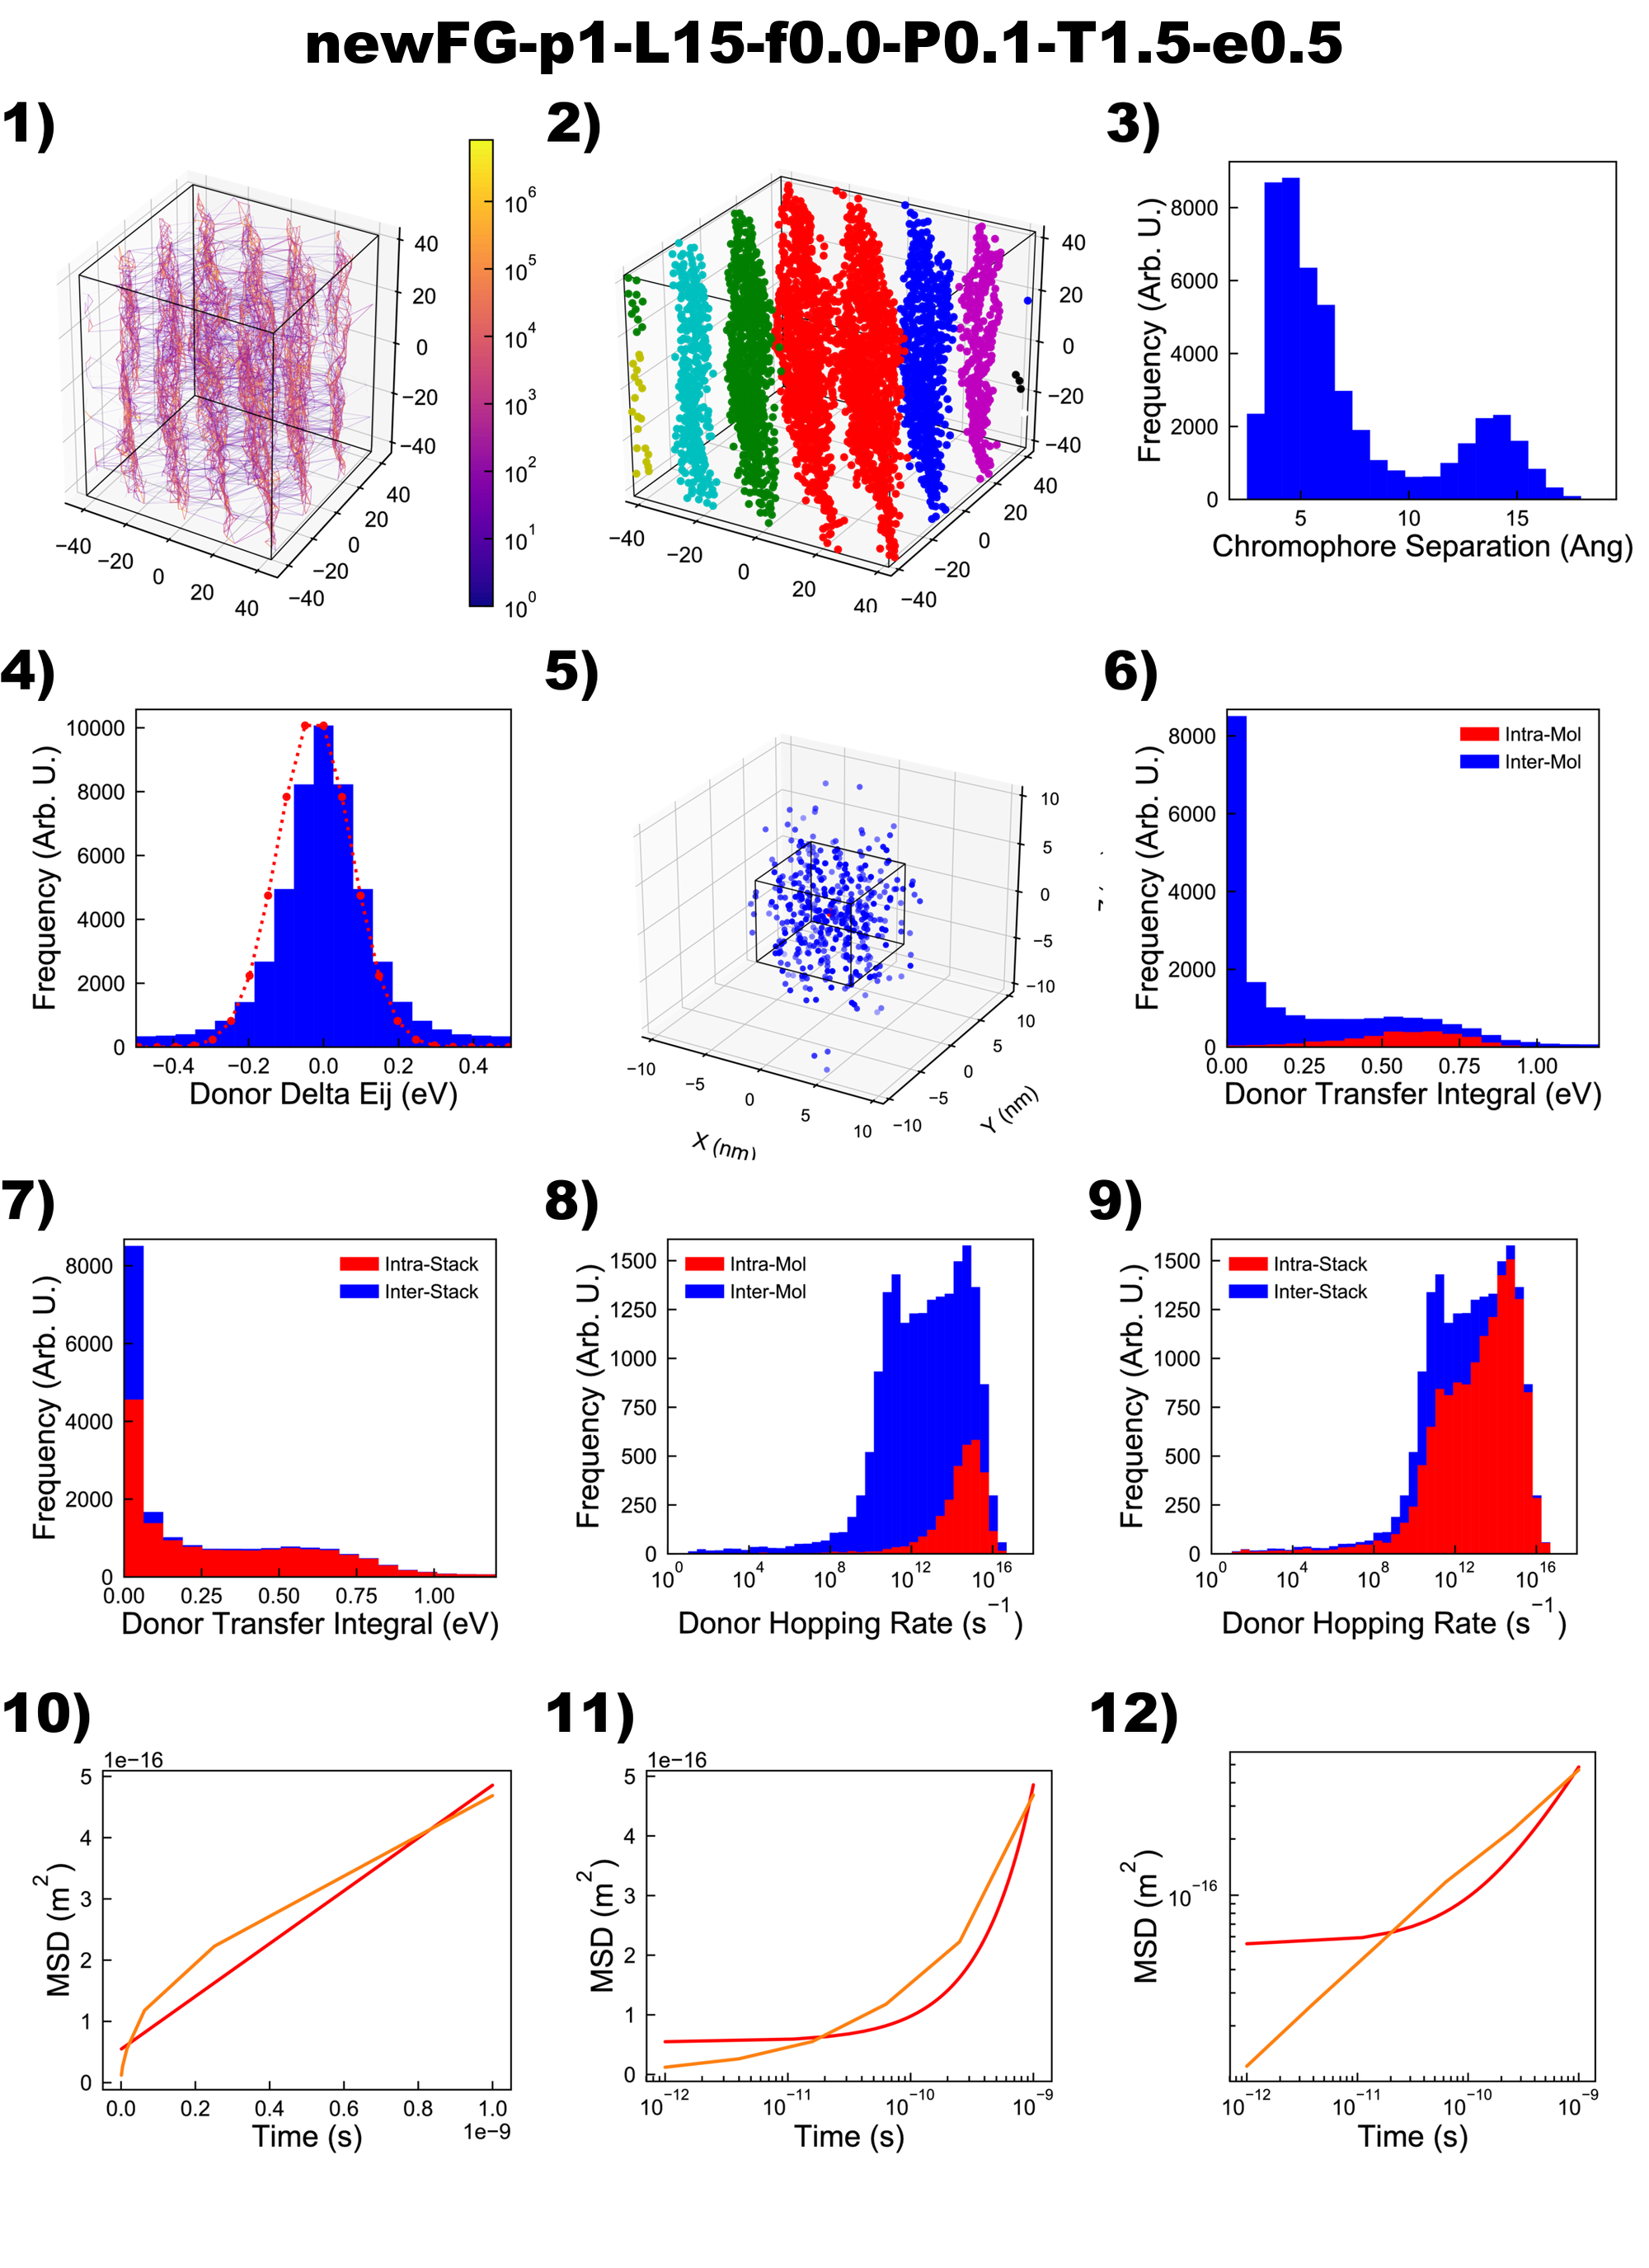
\includegraphics[width=0.85\textwidth]{Figures/newFG-p1-L15-f0.0-P0.1-T1.5-e0.5.png}
    \caption{   1) Chromophore connectivity network, 
                2) Location of `stacks', 
                3) Distribution of connected chromophore separations (defines stacks),
                4) Density of states of Frontier molecular orbital (delta Eij),
                5) KMC Carrier termination locations (defines anisotropy),
                6) Histogram of molecular transfer integrals,
                7) Histogram of stack transfer integrals,
                8) Histogram of molecular hopping rates,
                9) Histogram of stack hopping rates,
                10) Linear MSD plot,
                11) Semi-log-x MSD plot,
                12) Logarithmic MSD plot.}
	\label{fig:noMapT1.5}
\end{figure}


\begin{figure}[h]\centering
	\includegraphics[width=0.85\textwidth]{Figures/newFG-p1-L15-f0.0-P0.1-T1.75-e0.5.png}
    \caption{   1) Chromophore connectivity network, 
                2) Location of `stacks', 
                3) Distribution of connected chromophore separations (defines stacks),
                4) Density of states of Frontier molecular orbital (delta Eij),
                5) KMC Carrier termination locations (defines anisotropy),
                6) Histogram of molecular transfer integrals,
                7) Histogram of stack transfer integrals,
                8) Histogram of molecular hopping rates,
                9) Histogram of stack hopping rates,
                10) Linear MSD plot,
                11) Semi-log-x MSD plot,
                12) Logarithmic MSD plot.}
	\label{fig:noMapT1.75}
\end{figure}


\begin{figure}[h]\centering
	\includegraphics[width=0.85\textwidth]{Figures/newFG-p1-L15-f0.0-P0.1-T2.0-e0.5.png}
    \caption{   1) Chromophore connectivity network, 
                2) Location of `stacks', 
                3) Distribution of connected chromophore separations (defines stacks),
                4) Density of states of Frontier molecular orbital (delta Eij),
                5) KMC Carrier termination locations (defines anisotropy),
                6) Histogram of molecular transfer integrals,
                7) Histogram of stack transfer integrals,
                8) Histogram of molecular hopping rates,
                9) Histogram of stack hopping rates,
                10) Linear MSD plot,
                11) Semi-log-x MSD plot,
                12) Logarithmic MSD plot.}
	\label{fig:noMapT2.0}
\end{figure}


\begin{figure}[h]\centering
	\includegraphics[width=0.85\textwidth]{Figures/newFG-p1-L15-f0.0-P0.1-T2.25-e0.5.png}
    \caption{   1) Chromophore connectivity network, 
                2) Location of `stacks', 
                3) Distribution of connected chromophore separations (defines stacks),
                4) Density of states of Frontier molecular orbital (delta Eij),
                5) KMC Carrier termination locations (defines anisotropy),
                6) Histogram of molecular transfer integrals,
                7) Histogram of stack transfer integrals,
                8) Histogram of molecular hopping rates,
                9) Histogram of stack hopping rates,
                10) Linear MSD plot,
                11) Semi-log-x MSD plot,
                12) Logarithmic MSD plot.}
	\label{fig:noMapT2.25}
\end{figure}


\begin{figure}[h]\centering
	\includegraphics[width=0.85\textwidth]{Figures/newFG-p1-L15-f0.0-P0.1-T2.5-e0.5.png}
    \caption{   1) Chromophore connectivity network, 
                2) Location of `stacks', 
                3) Distribution of connected chromophore separations (defines stacks),
                4) Density of states of Frontier molecular orbital (delta Eij),
                5) KMC Carrier termination locations (defines anisotropy),
                6) Histogram of molecular transfer integrals,
                7) Histogram of stack transfer integrals,
                8) Histogram of molecular hopping rates,
                9) Histogram of stack hopping rates,
                10) Linear MSD plot,
                11) Semi-log-x MSD plot,
                12) Logarithmic MSD plot.}
	\label{fig:noMapT2.5}
\end{figure}


\clearpage


\bibliography{refs}
\bibliographystyle{unsrt}


\end{document}
